% Copyright (c)  2005-2010 EDF-EADS-PHIMECA.
% Permission is granted to copy, distribute and/or modify this document
% under the terms of the GNU Free Documentation License, Version 1.2
% or any later version published by the Free Software Foundation;
% with no Invariant Sections, no Front-Cover Texts, and no Back-Cover
% Texts.  A copy of the license is included in the section entitled "GNU
% Free Documentation License".

This section deals with the analysis of the requirements that guided the general implementation choices for the \OT\ platform. The system is here to be seen from a rather generic, functional point of view; it mainly consists in blocks handling the main functions of the platform. We shall detail the fundamental concepts that arise from the requirements and their role within the system.

At this stage of modeling, technical considerations shall not (except in specific cases) be addressed yet. The platform is seen as a system made up of components interacting with each other, providing designated functions. In this section, we shall answer the question "What does the system actually perform ?"

\section{Description of the analysis approach}

The \OT\ project aims at producing a risk analysis tool. When the project started, there was no equivalent tool available on the market, whether it be proprietary or Open Source software. Therefore, a choice was made to design an entirely new tool "from scratch", beginning with the requirements analysis, using the most effective methods and the most up-to-date scientific concepts, relying on tools widely recognized by the scientific community.

Considering the recent progress in computer science and software engineering, the platform will be implemented using an object-oriented language, which naturally leads us to use an object modeling approach to analyze and design the elements that will make up the code. The UML approach was therefore chosen for this preliminary stage of the project.

Readers interested in UML will find more detailed information in the guide written by Pierre-Alain Muller \cite{UML}. However, we will sum up the approach to present all the notions relevant to this document.

UML relies on the analysis of the requirements expressed by the future platform users, using a standard graphical formalism. Everything starts with the definition of use-cases that describe how the users will interact with the system. There can be several users (sometimes several thousands) but only their role regarding the system is taken into consideration. These users are supposed to describe the actions they want to perform and the responses they expect from the system. Therefore, at this stage of modeling, the actual realization ("how") of actions is not taken into account; only the functional need of the user ("what") is being considered.

First, these use cases are graphically modeled with ellipses, the users being represented as human figures (as shown in Figure \ref{fig:usecase}).

\begin{figure}[htb]
  \begin{center}
    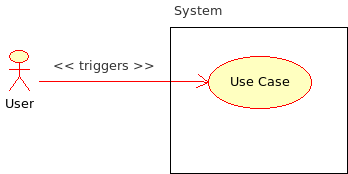
\includegraphics[scale=0.9]{Figures/analysis/usecase.png}
    \caption{Example of a use case triggered by a system user.}\label{fig:usecase}
  \end{center}
\end{figure}

All of the use cases triggered by the same user allow us to have an overview of the actions this user can carry out on the system.

Conversely, requiring all the users to describe the same use case allows us to study the case from multiple angles and to determine all the interactions that need to be taken into account between users.

Naturally, the definition of a use case is not limited to putting a designation within an ellipse. This description is only used to provide an overview of the use case. The use case must be described in detail: most often, this stage uses a natural language (i.e. free format) description of the user's actions and the system's responses. If this description requires highly technical content (which is the case for the \OT\ platform), it may be wiser to use a language close to either the user's requirements or the target system. The appendix provides an extensive description of the use cases (in algorithmic form) written for the \OT\ platform.

Based on these detailed descriptions, we can now extract concepts that are fundamental for the system and link them so as to view their interactions, their functional proximity and the abstract ideas that can be derived from them. We refer to this set of concepts and links as an \emph{analysis model}.

It is then possible, based on these concepts, to create bricks of variable size encompassing related notions, and thus to show the logical and functional view of the platform. This global view of the platform is essential to have a general understanding of the system as well as to consider its evolution capabilities.

The present chapter describes the results of this analysis, which was carried out with and for the platform users. In the next chapter, we will rely on this analysis to introduce the design model and the software architecture.

\section{Requirements analysis and use cases}

Interviews with the future users of the system have uncovered the following general requirements:
\begin{itemize}
\item the platform must allow the users to carry out uncertainty and risk analysis studies as well as statistically process data provided both internally and externally;
\item the platform must be of ergonomic and easy use for novice users, as well as complete and precise for expert users. It must therefore follow the Methodological Reference \cite{OTmeth} provided by EDF R\&D;
\item the platform must provide a graphical user interface (GUI) as well as a text user interface (TUI); it must also provide a means of external control by another code (\emph{scripting} and \emph{batch});
\item the platform must be efficient in order to handle several millions (or more) of computations, and must be able to use the distributed computing capabilities of an heterogenous network or a remote computer;
\item the platform must run in a Unix-like environment, but future ports to other environments (Windows, etc.) will be considered;
\item the platform is generic and must be able to interface with (almost) any field specific code;
\item the platform is developed using Open Source software and will be distributed under the terms of an Open Source license;
\item the platform includes efficient scientific methods that can be expanded or supplemented;
\item the platform uses Open Source tools that are considered as references in the field of statistics and optimization;
\item the platform will be primarily developed using object-oriented technologies;
\item the platform must be able to run either as a \emph{standalone} application or as an extension to another application;
\item the platform must interface with an indexed storage system that allows the preservation of results coming from previous computations, so as to avoid having to compute them again;
\item the platform must include an extensive online documentation.
\end{itemize}

These general requirements are described with more details in the use cases, which are grouped in packages according to the recommendations given in the Methodological Reference.

\subsection{Definition of the actors involved with the \OT\ platform}

The analysis of the actors involved with the \OT\ platform brings us to the following list:
\begin{itemize}
\item \emph{User}: this actor carries out the uncertainty treatment studies with the platform. From a practical point of view, it is the main actor which we will focus on, since the platform is being developed with that role in mind. It is in most cases a human being that will be interacting with the system, but other systems can also play that role in automated running modes (\emph{scripting} and \emph{batch}).
\item \emph{Developer}: this actor adds new functions to the \OT\ platform. Although the platform does not focus on this actor, it is implemented so as to make the development and integration tasks as easy as possible for them. It is always a human being.
\item \emph{Administrator}: this actor sets up the \OT\ platform on the target network. Their role is to configure the platform so that it provides the expected services. It is always a human being.
\item \emph{External code}: this actor is the field specific code that will be called upon in an uncertainty study. From the system's point of view, it is a passive actor.
\item \emph{Storage system}: this actor is the system that allows the preservation of results coming from previous studies. From the system's point of view, it is also a passive actor.
\end{itemize}

\subsection{Modeling package}

This package gathers all the use cases involved in defining an uncertainty treatment study before any computation is actually carried out by the system. Figure \ref{fig:modeling} details these use cases.

\begin{figure}[htb]
  \begin{center}
    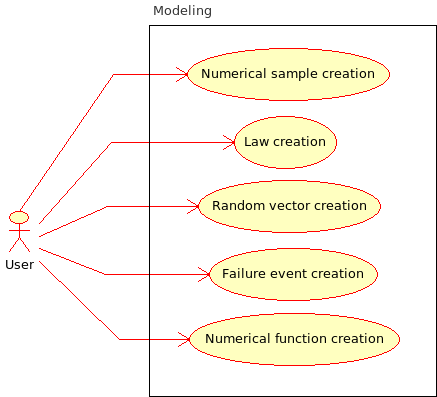
\includegraphics[scale=0.9]{Figures/analysis/modeling.png}
    \caption{Modeling use cases.}\label{fig:modeling}
  \end{center}
\end{figure}

The only actor involved in this package is the \emph{user}.

For the detailed use cases, please refer to the appendix.

\subsubsection{Creating a numerical sample}

The numerical sample is a key concept for the \OT\ platform, particularly with regards to its statistical capabilities. The user can create a sample in the system in different ways:
\begin{itemize}
\item by importing a file containing the description of the sample;
\item by manually setting the values of the sample through the interface;
\item by using a random variable to produce the sample;
\item by extracting a subsample from a given sample or expanding\footnote{In the case of the non parametric bootstrap, elements of a sample are randomly drawn to create a larger sized sample.} a given sample into a larger one.
\end{itemize}

\subsubsection{Creating a distribution}

The distribution is probably the core concept of the \OT\ platform. The uncertainty treatment model is, for the most part, based on the notion of distribution. A distribution can be created in different ways:
\begin{itemize}
\item by setting its parametric type and parameters through the interface;
\item by automatically establishing its parameters based on a numerical sample and a hypothesis on its type (distribution inference);
\item by combining other distributions (mixture distribution, assembly distribution);
\item by extracting a sub-section of a given distribution;
\item by creating the distribution from other distributions and numerical functions.
\end{itemize}

\subsubsection{Creating a random vector}

The random vector represents the concept of random variable within the \OT\ platform. It is the concept most easily manipulated by users in their studies. It can be created as follows:
\begin{itemize}
\item by setting its joint distribution;
\item by combining several other random vectors;
\item by extracting a sub-vector from a given random vector, or expanding a given random vector into a larger one;
\item by creating the vector from other random vectors and numerical functions.
\end{itemize}

\subsubsection{Creating a failure event}

A failure event is used to identify the limit state of a numerical function. It can be created very easily with a random vector, a threshold (in the form of a point) and a comparison operator that will compare the value of the vector with the one of the threshold.

\subsubsection{Creating a numerical function}

The numerical function is, along with the distribution, another core concept of the \OT\ platform. The numerical function represents the physical or theoretical model that is to be studied and through which the uncertainties on the input random vector will be propagated. This numerical function can be given in an analytical form or in a coded form (in which case it is defined within a external code).

\subsection{Propagation Package}

This package encompasses all the use cases that appear after modeling, when the user wants to propagate uncertainty through the external code. Figure \ref{fig:propagation} details these use cases.

\begin{figure}[htb]
  \begin{center}
    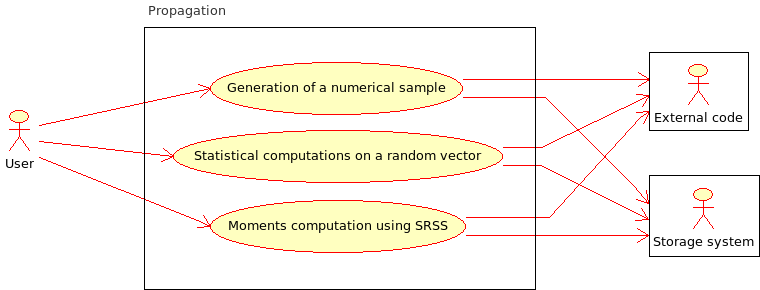
\includegraphics[scale=0.5]{Figures/analysis/propagation.png}
    \caption{Propagation use cases.}\label{fig:propagation}
  \end{center}
\end{figure}

In all use cases from this Propagation package, two new actors appear beside the user: the external code and the storage system. From the system's point of view, the external code behaves as a numerical function on which an uncertainty study is to be carried out. The storage system, which is important but optional, acts as a replacement for the external code during the (costly) evaluation of the numerical function.

The use cases are detailed in the appendix.

\subsubsection{Generating a numerical sample}

Generating a numerical sample means applying the numerical function on the input numerical sample. The generated sample is the numerical sample produced as an output of the numerical function. The samples can reach very large sizes (several million points) and therefore, the evaluation of the numerical function needs optimization. This can be achieved either by computing only the points that have not been computed yet, which makes use of the storage system; or by distributing the external code's execution on a computer network. The propagation of uncertainty based on Monte-Carlo methods belongs to this application field.

The distributed computing system being integrated in the \OT\ platform, it was decided not to represent it as an external actor.

\subsubsection{Statistical computations on a random vector}

The goal of an uncertainty processing study is to evaluate a given number of statistics on a random vector, which is generally defined as the output of a numerical function. The nature of these statistics may vary: mean value, standard deviation, threshold-crossing probability, and so on.

Depending on the statistics chosen, different algorithms can be implemented, which influences the number of calls on the numerical function and its derivative functions. As a direct corollary, the external code can be called a very large number of times, which results in an important computational overload that needs to be distributed throughout the network in order to reduce the waiting time for the user: an example of this would be the computation of the numerical function's gradient using the finite-difference method.

A storage system that is external to the platform and works as a cache can help reduce the number of computations by preserving the already computed results.

\subsubsection{Computing the moments using SRSS}

Computing moments using SRSS involves evaluating the numerical function, its gradient and its higher order derivatives. As for the computation of a threshold-crossing probability, it is sometimes necessary to evaluate the numerical function's derivatives using a finite difference algorithm, which requires the parallelization of the computations and the use of a storage system to preserve previous results.

\subsection{Prioritization Package}

The prioritization is the last stage in the uncertainty processing procedure, which evaluates the sensitivity of the output with respect to the input parameters. It comes after the propagation stage (see the previous section).

\begin{figure}[htb]
  \begin{center}
    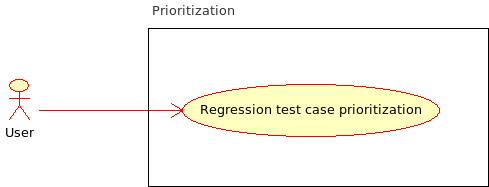
\includegraphics[scale=0.8]{Figures/analysis/prioritization.png}
    \caption{Prioritization use cases.}\label{fig:prioritization}
  \end{center}
\end{figure}

The use cases are detailed in the appendix.

\subsubsection{Regression test case prioritization}

Prioritization uses a linear regression computation between the input and output parameters of the numerical function evaluated during the propagation stage, so as to assess the sensitivity of the output parameters regarding the input. This stage usually makes use of the platform's graphical abilities in order to visualize the results.

\subsection{Contribution package}

This package encompasses the use cases dealing with the development and integration of new functionalities into the \OT\ platform.

\begin{figure}[htb]
  \begin{center}
    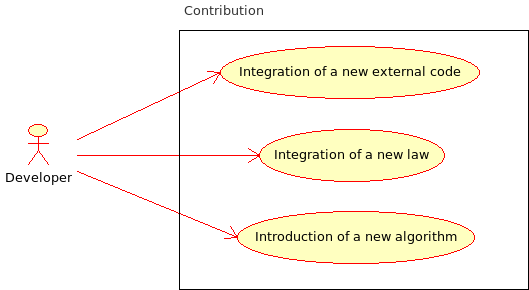
\includegraphics[scale=0.7]{Figures/analysis/contribution.png}
    \caption{Contribution use cases.}\label{fig:contribution}
  \end{center}
\end{figure}

As shown in Figure \ref{fig:contribution}, a new actor, the developer, is involved and can be competent in one or several of the following fields:
\begin{itemize}
\item Computer science
\item Numerical analysis
\item Statistics/probabilities
\end{itemize}

Several persons may be needed to combine all of the above skills. Integrating new functions into the \OT\ platform may require the collaboration of several people.

These use cases are not detailed in this document; they will however be introduced as documented examples provided with the platform distribution.

\subsubsection{Integrating a new external code}

The external code is the passive actor that supports the notion of numerical function; integrating new functions into the platform therefore requires interfacing with a field-specific code, using an API that the code must follow. If it is not natively the case, an interface layer between the API and the code needs to be developed. This layer is not the responsibility of the \OT\ platform. The platform only defines the API that enables communication with the external code.

\subsubsection{Integrating a new distribution}

Integrating new distributions in the platform enhances its modeling capabilities. The standard distributions included in the platform are described in the project's Methodological Reference [OTmeth].

\subsubsection{Integrating a new algorithm}

Integrating new algorithms in the platform enhances its modeling and computing capabilities. The standard algorithms included in the platform are described in the project's Methodological Reference [OTmeth].

\subsection{Configuration package}

This package encompasses the use cases related to the platform's setup on a computer park for a field-specific use.

\begin{figure}[htb]
  \begin{center}
    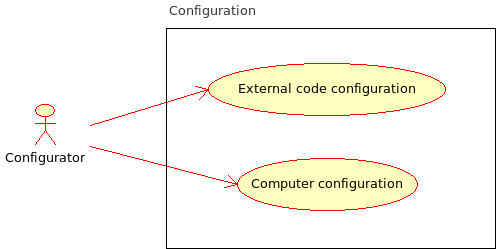
\includegraphics[scale=0.8]{Figures/analysis/configuration.png}
    \caption{Configuration use case.}\label{fig:configuration}
  \end{center}
\end{figure}

The configurator (shown in Figure \ref{fig:configuration}) acts as the person responsible for the installation and administration of the platform. They set up the connection between the external codes and \OT, and configure the platform's networking parameters. It is a static configuration: there is no automatic exploration of the computing environment.

These use cases are not detailed in this document; they will however be introduced as documented examples provided with the platform distribution.

\subsubsection{External code configuration}

Configuring external codes requires the configurator to define which data sets of the external code are related to the current uncertainty study, to state in the platform which external code is to be used and which of its parameters are considered uncertain.

\subsubsection{Computer configuration}

The computers' configuration is carried out by the configurator; a configuration states which computing resources are available for the execution of the platform and of its dependencies (external code, storage system, and so on), as well as the protocols, identifiers, priorities, et. related to these resources.

\section{Description of the analysis concepts}

Writing the use cases in a detailed form allows us to shed light on the concepts the user wishes to manipulate through the platform. These concepts are linked with one another by relationships such as "depends", "uses", "combines" ("aggregates", "composes"), "generalizes", "specializes", and so on. The following section shows the UML notational system (for more information, please refer to \cite{UML}) that was used, in order to make the graphs easier to understand.

In the analysis model, these concepts are abstract entities that do not necessarily have a direct projection as a programming entity (object, class,...). Their role is to clear the vision one can have of the system and of its internal mechanism. No technical considerations should normally appear at this stage of modeling. However, a technical consideration may exceptionally be taken into account at the analysis level if it should have nefarious consequences on the model.

\label{notations}\subsection{Notations used in the analysis model}

This section briefly describes the visual representation of the concepts and of the relationships that link them.

\subsubsection{Concept}

The concept is an entity manipulated by the system's user, who has an intellectual representation of the concept. Its symbol is a rectangle containing the name of the concept. Figure \ref{fig:linking_concepts} shows six concepts A, B, C, D, E, and F, linked with one another.

\begin{figure}[htb]
  \begin{center}
    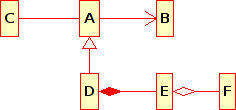
\includegraphics[scale=0.9]{Figures/analysis/linking_concepts.png}
    \caption{Graphical representation of concepts from an analysis model and their relationships.}\label{fig:linking_concepts}
  \end{center}
\end{figure}

\subsubsection{Association}

Association defines a relationship of reciprocal use between two concepts. In the example given in Figure \ref{fig:linking_concepts}, the concepts A and C are linked by an association. Associations are represented by full lines linking the concept boxes. Association is bidirectional: A knows C and C knows A.

\emph{Example}: consider the concepts Vector and Distribution; we can say that a Vector may be associated to a Distribution, and vice versa.

\subsubsection{Unidirectional association}

This association type is a restriction of the more general association, which allows flow in only one direction. This is the case for concepts A and B of our example: A knows B but B does not know A.

\emph{Example}: consider the concepts Vector and Sample; we can say that a Vector may be associated to a Sample (a Vector can produce a Sample) but a Sample cannot be associated to a Vector.

\subsubsection{Generalization/Specialization}

This relationship links two concepts, one of them (A) being more general than the other (D). We can also revert the reading of the link and say that one of them (D) is more specialized than the other (A). Its graphical representation is a hollow arrow pointing to the more general concept.

\emph{Example}: a Distribution is more general than a UsualDistribution, whereas a UsualDistribution is more specialized than a Distribution.

\subsubsection{Aggregation}

Aggregation is the relationship that links a container concept to a contained concept. Its graphical representation is a clear diamond shape on the containing concept end of the relationship.

\emph{Example}: a Sample is a collection or aggregation of Points.

\subsubsection{Composition}

Composition is a restriction of Aggregation which introduces a life cycle dependency: contained concepts exist only for the container and within the container's lifespan; conversely, the container exists only if the containees also exist. Its graphical representation is a black diamond shape on the container end of the relationship.

\emph{Example}: a MixtureDistribution is a composition of WeightedDistributions, each characterized by its scalar weight.

\subsubsection{Multiplicity of associations}

Each end of the association may have a multiplicity indicating the number of instances of the concept (that is, the number of real objects belonging to this concept) simultaneously existing for each instance of the facing concept. This multiplicity can have one of the following values:
\begin{itemize}
\item \emph{1}: one instance only;
\item \emph{n}: n instances (n positive integer);
\item \emph{m..n}: between m and n instances (m and n positive integers);
\item \emph{*}: any number of instances (0 included);
\item etc.
\end{itemize}

\emph{Example}: A Sample is a collection made up of any number of Points (multiplicity * regarding the Point concept).

\subsubsection{Role within an association}

Along with the multiplicity, each end of the association can carry a name that designates the role played by the concept regarding the concept at the other end of the association.

\emph{Example}: a Vector is associated to a Distribution. This Distribution (on its end of the association) is assigned the role of "joint distribution". Therefore the Distribution is a "joint distribution" for the Vector.

\subsubsection{Association's name}

Each association can have a name, generally taking the form of an action verb describing the association and the way it should be interpreted. If any disambiguation is required, it can be completed with an arrow indicating the direction for which the name makes sense.

\emph{Example}: a Vector "creates" a Sample, therefore the association carries the name "creation".

\subsection{Basic concepts}

These concepts are the foundation bricks on which more advanced concepts will rely.

\begin{figure}[htb]
  \begin{center}
    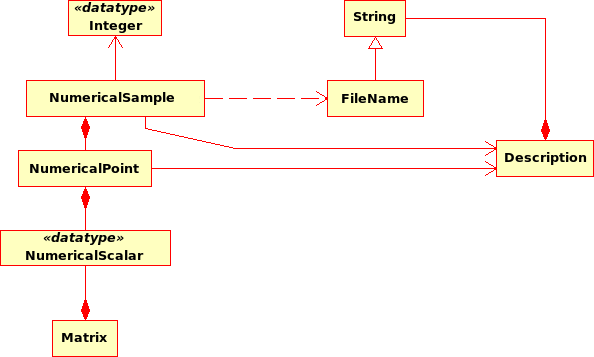
\includegraphics[scale=0.7]{Figures/analysis/basic_concepts.png}
    \caption{Basic concepts.}\label{fig:basic_concepts}
  \end{center}
\end{figure}

\subsubsection{Integer}

The integer is a basic type for the \OT\ platform. It stores a whole positive or zero numerical data. Mathematically, it is a natural number. It may be used to describe the size of a sample, the dimension of a vector, the rank of a matrix, etc.

\subsubsection{NumericalScalar}

The NumericalScalar is another base type. It contains a numerical data that can be used in an uncertainty computation. Mathematically, it is a real number.

\subsubsection{String}

The String is a basic type that stores a text data of any length.

\subsubsection{FileName}

The FileName is a type derived from String specialized in the storage of filenames. Its syntax must correspond to a valid expression of a relative or absolute path to a file or directory on the disk.

\subsubsection{NumericalPoint}

The NumericalPoint is an elementary type made up of NumericalScalars. It covers the mathematical notion of a point in a multi-dimensional space, and once it is instantiated, its value remains constant. It can be used as a realization of a vector, mean value of a sample, etc. Its behavior is strictly deterministic.

The NumericalPoint gives access to its components. The NumericalPoint can be linked to a Description that will represent the names of its components.

\subsubsection{Description}

The Description is an elementary type made up of Strings. Its role is to provide a name or a description for an ordered set the same size as the Description. It can be associated with a NumericalPoint or a RandomVector to describe its components, with a NumericalSample to describe its points, etc.

\subsubsection{NumericalSample}

The NumericalSample is an elementary type made up of NumericalPoints. It is an homogeneous collection of points that have the same dimension. It covers the mathematical notion of a set of points. Given the multi-dimensional aspect of the points, the NumericalSample is also multi-dimensional. Its behavior is also deterministic. It can be used as a sample from a vector.

The NumericalSample gives access to its elements.

\subsubsection{Matrix}

The Matrix (see Figure \ref{fig:matrix}) is an elementary type made up of NumericalScalars. It covers the mathematical notion of a matrix in its most general form (rectangular, asymmetric, etc.). The Matrix has a deterministic behavior. It can be specialized into more specific concepts such as square matrices, symmetric matrices, covariance matrices, etc.

\begin{figure}[htb]
  \begin{center}
    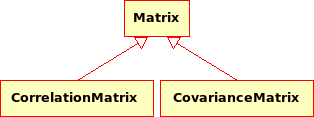
\includegraphics[scale=0.9]{Figures/analysis/matrix.png}
    \caption{Matrix concepts.}\label{fig:matrix}
  \end{center}
\end{figure}

\subsection{Uncertainty concepts}

\subsubsection{RandomVector}

The RandomVector (see Figure \ref{fig:random_vector}) is, from the user's point of view, the core concept. It covers both the mathematical notion of random vector and the programming concept of variable. It is essentially a multi-dimensional object, which means it always has a dimension (even if this dimension is 1). As a corollary, \emph{there is no notion of random scalar}: within the platform, such an object is represented by a random vector whose dimension is 1.

\begin{figure}[htb]
  \begin{center}
    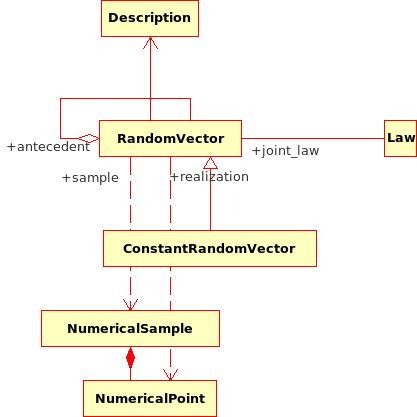
\includegraphics[scale=0.9]{Figures/analysis/random_vector.png}
    \caption{The concept of random vector.}\label{fig:random_vector}
  \end{center}
\end{figure}

The RandomVector is always associated with a Distribution called a joint distribution. This distribution models the vector's uncertain behavior. The RandomVector can be derived into a ConstantRandomVector whose realization is deterministically always the same NumericalPoint. The RandomVector can produce a NumericalPoint called realization and a NumericalSample called sample.

The RandomVector can be created from other RandomVectors; therefore there is a reflexive aggregation of the concept on itself, which bears the name \emph{antecedent} on the thus created RandomVector end, so as to allow the created RandomVector to find its antecedents through the creation process. In other words, this mechanism allows a RandomVector $Y = f(X)$ (where X is the antecedent RandomVector of Y) to identify X and (if the RandomVector definitions are chained) all of the previous antecedents up to the first RandomVector.

\subsubsection{FailureEvent}

The FailureEvent (see Figure \ref{fig:failure_event}) is a concept that allows to define the limite state of a RandomVector "vector" with respect to a NumericalPoint "threshold", depending on a comparison operator "operator".

\begin{figure}[htb]
  \begin{center}
    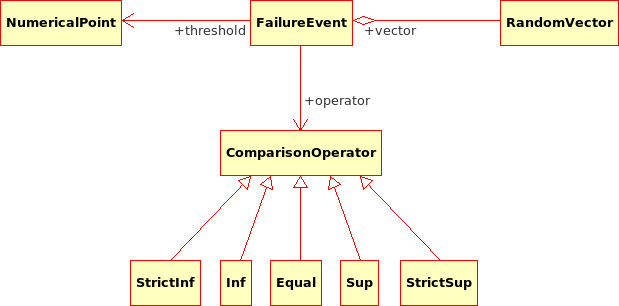
\includegraphics[scale=0.6]{Figures/analysis/failure_event.png}
    \caption{The concept of failure event.}\label{fig:failure_event}
  \end{center}
\end{figure}

\subsubsection{Distribution}

From the modeling point of view, the Distribution is the core concept. It is the richest concept that encompasses most of the notions related to the treatment of uncertainties, as shown in Figure \ref{fig:distribution}. The distribution is at the crossroads of the deterministic and uncertain domains. Like the other concepts of the platform, it is a multi-dimensional concept.

The previous section about the RandomVector already showed the relationship that links it with the Distribution: each RandomVector is defined by a joint Distribution. This Distribution can in turn be derived into UsualDistribution, FunctionalDistribution, MixtureDistribution and AssemblyDistribution.

\begin{figure}[htb]
  \begin{center}
    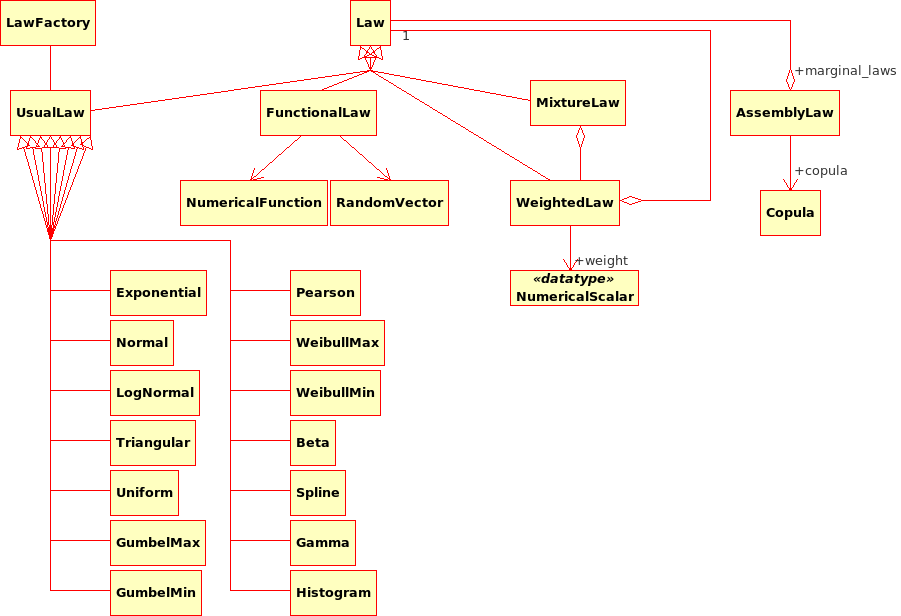
\includegraphics[scale=0.5]{Figures/analysis/distribution.png}
    \caption{The concept of uncertain distribution.}\label{fig:distribution}
  \end{center}
\end{figure}

\subsubsection{UsualDistribution}

The UsualDistribution is the basic brick for the Distribution concept. The concept of UsualDistribution can in turn be derived into various distributions: Exponential, Normal, LogNormal, Triangular, Uniform, GumbelMax, GumbelMin, Pearson, WeibullMax, WeibullMin, Beta, Spline, Gamma and Histogram. To each distribution corresponds an analytical formula describing the exact behavior of the said distribution. These distributions are by definition multi-dimensional. However, in some cases, there is not always an analytical formulation for all of the dimensions. The implementation will therefore not be able to cover all possibilities.

\subsubsection{AssemblyDistribution}

When a UsualDistribution cannot be directly defined for a RandomVector of a given dimension, either because the distribution is unknown, or does not exist, or for any other reason, it is possible to combine Distributions describing the marginal distribution of the RandomVector with the help of a Copula, which determines the dependency structure of this RandomVector. The Distribution assembly mechanism is supported by the concept of AssemblyDistribution. The aggregation of Distributions (called marginal\_distributions) is ordered and has the same size as the RandomVector.

\subsubsection{WeightedDistribution}

The WeightedDistribution is an arbitrary Distribution associated with a NumericalScalar that serves as a weight value in a linear combination of Distributions. Each WeightedDistribution is associated with a unique Distribution for which it defines a weight.

\subsubsection{MixtureDistribution}

The MixtureDistribution is a concept defining a linear combination of Distributions. It is modeled as an aggregation of WeightedDistributions, whose underlying relationship is the sum; each WeightedDistribution brings the weight of the Distribution in the linear combination. The mathematical definition requires the \emph{weights} to belong to the [0,1] interval and their sum to be 1.

Like all Distributions, the MixtureDistribution is a multi-dimensional concept and de facto requires the aggregation to include same-size Distributions only.

\subsubsection{FunctionalDistribution}

The FunctionalDistribution is the Distribution resulting from a RandomVector being passed to a NumericalFunction. This sort of Distribution cannot be precisely defined in the general (non analytical) case, therefore the FunctionalDistribution is determined by the input parameters that define it.

\emph{NB: it was decided to use the RandomVector rather than its joint distribution, because the RandomVector (contrary to the Distribution) can access all of its antecedents. This history of antecedents is also necessary to define the Distribution.}

\subsubsection{DistributionFactory}

The DistributionFactory is a concept whose need arises during the design stage. It answers the need to designate a Distribution by its type when a Distribution-type object designates a specific instance (on this topic, refer to section \ref{factory}; for more details, see \cite{GoF}). The DistributionFactory therefore designates a family of Distributions. It is an abstract concept that needs to be derived into concrete sub-concepts such as ExponentialFactory, NormalFactory, and so on, as many times as there are concrete instantiable classes.

\begin{figure}[htb]
  \begin{center}
    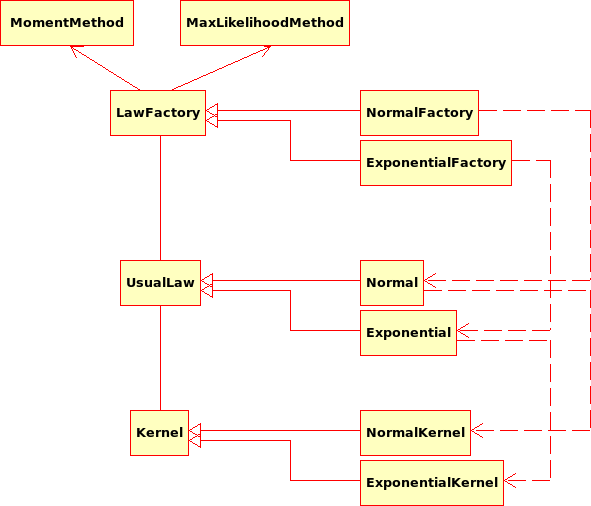
\includegraphics[scale=0.7]{Figures/analysis/distribution_family.png}
    \caption{The concept of distribution family.}\label{fig:distribution_family}
  \end{center}
\end{figure}

Therefore, to each specialized UsualDistribution corresponds a specialized DistributionFactory that can instantiate a specialized object: NormalFactory corresponds to Normal, ExponentialFactory to Exponential, and so on. NormalFactory can produce any Normal distribution, ExponentialFactory can produce any Exponential distribution, and so on for any other UsualDistribution: DistributionFactory therefore covers the mathematical concept of a distribution family.

The DistributionFactory can produce Distributions in different ways, therefore the concept is linked to the MomentsMethod and MaxLikelihoodMethod concepts. Both provide the algorithms needed to produce distributions.

\subsubsection{Kernel}

On top of the distribution family notion supported by the concept of DistributionFactory, it is necessary to have a specific instance of each UsualDistribution at one's disposal. In a way, this instance represents the generator for the distribution family. This specific instance is described by the Kernel concept. Each UsualDistribution can generate its Kernel: therefore a Normal generates NormalKernel, Exponential generates ExponentialKernel, and so on.

\subsection{Function concepts}

\label{numericalfunction}\subsubsection{NumericalFunction}

The NumericalFunction is the concept covering the notion of mathematical function. It is an entity that takes a NumericalPoint as input and produces a NumericalPoint as output. The dimensions of both NumericalPoint can differ.

\begin{figure}[htb]
  \begin{center}
    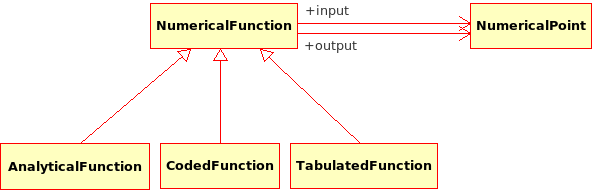
\includegraphics[scale=0.6]{Figures/analysis/numerical_function.png}
    \caption{The concept of numerical function.}\label{fig:numerical_function}
  \end{center}
\end{figure}

The NumericalFunction can be derived into AnalyticalFunction, CodedFunction and TabulatedFunction. The analysis is not directly concerned with these derived concepts, but they indirectly show:
\begin{itemize}
\item the link with the external code that the CodedFunction will have to support;
\item the need to have pre-wired functions within the platform (in the AnalyticalFunction);
\item the need for user-defined functions (TabulatedFunction).
\end{itemize}

\subsubsection{Copula}

The copula is the entity that covers the notion of mathematical copula. Mathematically speaking, it is as much a numerical function as the NumericalFunction; however, these concepts have been made distinct because they are used in very different contexts : the NumericalFunction is used in conjunction with RandomVectors and NumericalSamples, whereas the Copula is used only to define an AssemblyDistribution. Moreover, as we will see in the design model, this separation is emphasized by the operations required from each concept.

\subsection{Algorithm concepts}

\subsubsection{SimulationAlgorithm}

The SimulationAlgorithm is the concept covering all of the uncertainty propagation methods in the platform. It is an abstract concept that derives into sub-concepts such as MonteCarlo, FORM, SORM, SRSS, and so on. A SimulationAlgorithm produces a SimulationResult as output, which stores all the information needed for the prioritization stage.

\begin{figure}[htb]
  \begin{center}
    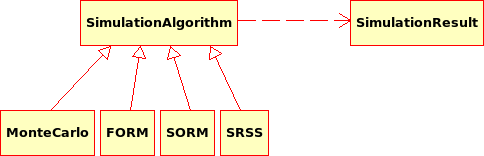
\includegraphics[scale=0.8]{Figures/analysis/simulation_algo.png}
    \caption{The concept of simulation algorithm.}\label{fig:simulation_algo}
  \end{center}
\end{figure}

\section{Synopsis of a functional architecture}

\subsection{Packages}

The tasks of modeling, analysis (described in this chapter) and design (described in next chapter) enable us to define concepts and objects closely related to one another. These will be grouped in the following packages:
\begin{itemize}
\item \emph{GUI}: this package encompasses all objects directly linked to the graphical interface (e.g. Qt objects);
\item \emph{Graphical objects}: this package encompasses all of the objects whose role is to adapt field-specific and technological objects into GUI objects. It can be seen as the graphical interface for field-specific objects (e.g. histograms, pie charts, graphs of functions, and so on);
\item \emph{TUI}: this package encompasses all the objects interfacing with field-specific objets for a text-based use of the platform (e.g. SWIG objects);
\item \emph{Procedures}: this package encompasses any processing that is not (or cannot) be modeled with field-specific or technological objects (e.g. conditional random vector). It also contains sequences that represent typical action chains frequently used in uncertainty treatment studies;
\item \emph{Uncertain objects}: this package encompasses objects and concepts linked to the modeling of field-specific data with uncertain variables (e.g. random vectors, distributions, etc.);
\item \emph{Simulation algorithms}: this package encompasses the various uncertainty propagation algorithms supported by the platform and the objects associated with the results (e.g. Monte-Carlo, FORM, SORM, etc.);
\item \emph{Statistical objects}: this package encompasses the objects and concepts associated with the statistical processing of field-specific data (e.g. sample);
\item \emph{Optimization functions}: this package encompasses the standard optimization methods needed for the simulation algorithms (e.g. SQP);
\item \emph{Basic numerical functions}: this package encompasses the mathematical and numerical functions standardly distributed with the platform (e.g. log, exp, sin, cos, etc.);
\item \emph{Basic classes}: this package encompasses the utility classes on which all of the higher level packages rely (e.g. String, FileName, Matrix, Tensor, etc.).
\end{itemize}

\subsection{Layers}

The previously introduced packages can also be grouped into software layers, each layer representing a different abstraction level of the \OT\ platform.

As can be seen in Figure \ref{fig:general_overview}, the layers can be stacked as follows:
\begin{itemize}
\item \emph{External services}: these are all the development prerequisites on which the platform relies, as well as the services offered by passive actors such as the external code or the storage system;
\item \emph{Basis brick}: it encompasses the packages offering core statistical and mathematical services for the platform;
\item \emph{Field-specific brick}: it is the essential layer that represents the core of the platform, in which are to be found packages responsible for the modeling and the propagation of uncertainties;
\item \emph{Sequences}: this layer assembles components from the field-specific brick to carry out complex uncertainty processing tasks;
\item \emph{User interface}: it is the layer responsible for the display and abstraction of field-specific objects into cognitively representable elements.
\end{itemize}

The perimeter of the \OT\ platform is the solid border that surrounds the four top layers. The bottom layer representing the external services does not strictly belong to the platform: it is made up of prerequisites that are not included in the developments and in the modeling.

Cutting out the functional architecture into layers like this has direct implications on the platform's development process: the top layers will have to be developed on the basis of the bottom layers. Therefore, the development will be carried out chronologically, from the bottom layers to the top ones. This does not mean that one layer has to be entirely finished before the development of the next one starts. However, the packages on which one layer relies will have to be at least partially developed before actually beginning the development of the said layer's packages.

\label{diagram}\subsection{General diagram}

\begin{figure}[htb]
  \begin{center}
    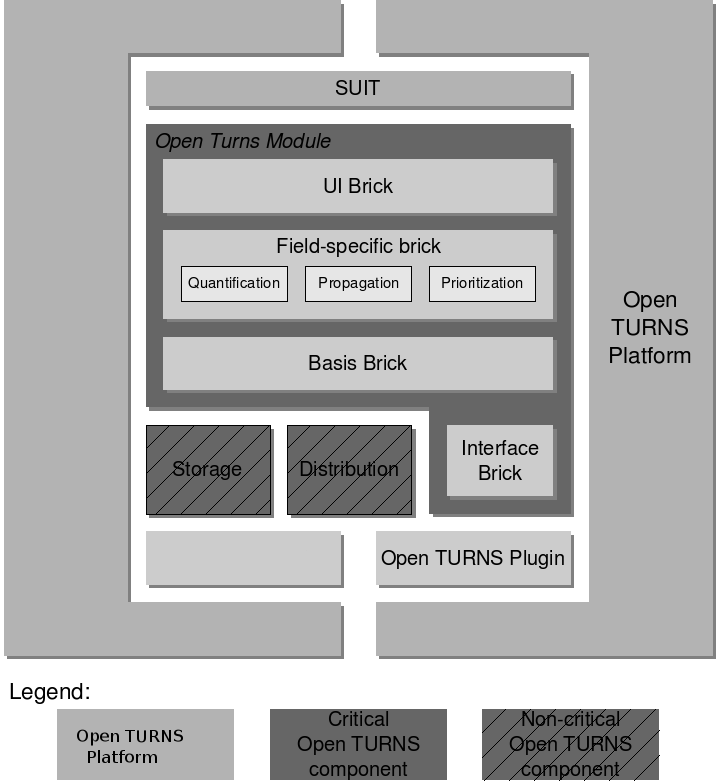
\includegraphics[scale=0.7]{Figures/analysis/general_overview.png}
    \caption{General diagram.}\label{fig:general_overview}
  \end{center}
\end{figure}

Figure \ref{fig:general_overview} shows the general diagram of the \OT\ platform and its brick structure:
\begin{itemize}
\item \emph{Interface brick}: used to provide communication with the operating system and the platform's prerequisites;
\item \emph{Basis brick}: basic components of the platform on which the functional, higher-level bricks rely;
\item \emph{Field-specific brick}: components used to model an uncertainty treatment study (quantization, propagation, prioritization, etc.);
\item \emph{UI brick}: components used to manipulate the platform and to visualize results.
\end{itemize}

The Storage service has the responsibility to store the computated data; the Distribution service's role is to distribute computations on a computer network. Both are considered non-critical: their development can be postponed in time in order to focus on the platform's core.

All of these elements make up the development perimeter within the \OT\ project.

The Plugin component is in charge of the communication between the platform and the external code. The platform will standardly offer a version providing a mechanism for generic communication with external codes, but aside from this version, the Plugin component is outside of the project's scope: its implementation is the responsibility of the external code, which will have to follow the API provided by \OT.


Figure \ref{fig:functional_diagram} describes the architecture of the \OT\ platform from a functional angle. It shows the packages resulting from the previously described concept groups, as well as other packages resulting from the design stage, the use cases or the general specifications of the platform. The layers are also represented as frames around the packages.

\begin{figure}[htb]
  \begin{center}
    \includegraphics[scale=0.7]{Figures/analysis/functional_diagram.png}
    \caption{Functional diagram.}\label{fig:functional_diagram}
  \end{center}
\end{figure}
